\documentclass{article}
\textheight 23.5cm \textwidth 15.8cm
%\leftskip -1cm
\topmargin -1.5cm \oddsidemargin 0.3cm \evensidemargin -0.3cm
%\documentclass[final]{siamltex}

\usepackage{verbatim}
\usepackage{fancyhdr}
\usepackage{graphicx}

%\pagestyle{fancy} \lhead{FDM Homework Template} \chead{}
%\rhead{\bfseries Yan XU}
%
%\lfoot{} \cfoot{} \rfoot{\thepage}
%\renewcommand{\headrulewidth}{0.4pt}
%\renewcommand{\footrulewidth}{0.4pt}
%

%利用TEX排版系统的CTEX中文套装
\usepackage[UTF8,noindent]{ctex}
%等式对齐
\usepackage{amsmath}
\usepackage{amssymb}

\title{ASAP与ARAP参数化}
\author{陈柯}

\begin{document}
	\maketitle
	
	\section{目的}
	
	1.	实现ASAP参数化
	
	2.  实现ARAP参数化
	
	\section{算法}
	\subsection{参数化的能量}
	对于3维网格中的每个三角形$x_t,t=1,\cdots,T$,都有一个自己局部的等距参数化
	$x_t=\{x_t^0,x_t^1,x_t^2\}$,可以理解为$x_t^j$就是一个三角形顶点的3维坐标。再设
	将其参数化后的各点为$u_t=\{u_t^0,u_t^1,u_t^2\}$,可以理解为$u_t^j$就是一个平面上
	的的2维坐标。在$x_t$到$u_t$之间的存在唯一的仿射变换,我们设该变换的 Jacobian 矩阵
	记为$J_t(u)$,它实际上代表了映射的线性变换的部分。在网格的参数化中,我们希望参数化
	保持了原网格的几何性质,也就是让这个Jacobian 矩阵性质足够好,或者说更加接近我们给予
	的一个矩阵,我们将其引入为辅助矩阵$L_t$,再定义能量:
	$$E(u,L)=\sum_{t=1}^{T}A_t\Vert J_t(u)-L_t\Vert_F^2$$
	其中$A_t$为三角形$x_t$的面积。这样我们就将参数化问题转化为了极小化能量$E(u,L)$的问
	题。上面的能量表达式也可以被重写为:
	$$E(u,L)=\frac{1}{2}\sum_{t=1}^{T}\sum_{i=0}^{2}\cot{(\theta_t^i)}
	\Vert(u_t^i-u_t^{i+1})-L_t(x_t^i-x_t^{i+1})\Vert^2$$
	其中$\theta_t^i$为三角形$x_t$中边$x_t^ix_t^{i+1}$所对的角。
	
	\subsection{ASAP参数化}
	取$L_t$为相似变换下的矩阵,即
	$L_t=\begin{pmatrix}   
		a_t&b_t\\-b_t&a_t
	\end{pmatrix},a_t,b_t\in\mathbb{R},t\in\{1,\cdots,T\}$。

	我们设$u_t^{i,k}-u_t^{i+1,k}=\Delta u_t^{i,k},k=0,1$,那么能量可表达为
	$$E(u,L)=\frac{1}{2}\sum_{t=1}^{T}\sum_{i=0}^{2}\cot{(\theta_t^i)}
	\left((\Delta u_t^{i,0}-a_t\Delta x_t^{i,0}-b_t\Delta x_t^{i,1})^2+
	(\Delta u_t^{i,1}+b_t\Delta x_t^{i,0}-a_t\Delta x_t^{i,1})^2\right)
	$$
	在能量中求$a_t,b_t$的偏导,可得:
	$$\frac{\partial{E}}{\partial{a_t}}=\sum_{i=0}^{2}\cot{(\theta_t^i)}
	\left(
	((\Delta x_t^{i,0})^2+(\Delta x_t^{i,1})^2)a_t-u_t^{i,0}\Delta x_t^{i,0}
	+u_t^{i+1,0}\Delta x_t^{i,0}-u_t^{i,1}\Delta x_t^{i,1}
	+u_t^{i+1,1}\Delta x_t^{i,1}
	\right)
	$$
	$$\frac{\partial{E}}{\partial{b_t}}=\sum_{i=0}^{2}\cot{(\theta_t^i)}
	\left(
	((\Delta x_t^{i,0})^2+(\Delta x_t^{i,1})^2)b_t-u_t^{i,0}\Delta x_t^{i,1}
	+u_t^{i+1,0}\Delta x_t^{i,1}+u_t^{i,1}\Delta x_t^{i,0}
	-u_t^{i+1,1}\Delta x_t^{i,0}
	\right)
	$$
	求$u_t^{i,0},u_t^{i,1}$的偏导,可得:
	$$\frac{\partial{E}}{\partial{u_{t_0}^{i_0,0}}}=\sum_{u_{t_0}^{i_0}\in u_t}
	\cot{(\theta_t^i)}(\Delta u_t^{i,0}-a_t\Delta x_t^{i,0}-b_t\Delta x_t^{i,1})
	-\cot{(\theta_t^{i-1})}(\Delta u_t^{i-1,0}-a_t\Delta x_t^{i-1,0}-b_t\Delta 
	x_t^{i-1,1})
	$$
	$$\frac{\partial{E}}{\partial{u_{t_0}^{i_0,1}}}=\sum_{u_{t_0}^{i_0}\in u_t}
	\cot{(\theta_t^i)}(\Delta u_t^{i,1}+b_t\Delta x_t^{i,0}-a_t\Delta x_t^{i,1})
	-\cot{(\theta_t^{i-1})}(\Delta u_t^{i-1,1}+b_t\Delta x_t^{i-1,0}-a_t\Delta 
	x_t^{i-1,1})
	$$
	令各偏导等于0,我们就可以构建稀疏方阵。再令首个边界上的起点和中点为固定点,分别固定
	到$(0,0)$和$(1,1)$,然后解出方程组即可。
	\subsection{ARAP参数化}
	取$L_t$为正交变换下的矩阵,即
	$L_t=\begin{pmatrix}   
		\cos{(\theta_t)}&\sin{(\theta_t)}\\-\sin{(\theta_t)}&\cos{(\theta_t)}
	\end{pmatrix},\theta_t\in[0,2\pi),t\in\{1,\cdots,T\}$。在这里我们采用
	“Local/Global”算法,也称迭代法来计算ARAP参数化。算法分3步:
	
	1.给网格一个初始的参数化,边界固定不固定无要求,只要每个三角形不翻转即可。本次我们
	采用ASAP参数化作为初始参数化
	
	2.Local Phase:对
	$$S_t(u)=\sum_{i=0}^{2}\cot{(\theta_t^i)}
	\begin{pmatrix}\Delta u_t^{i,0}\\\Delta u_t^{i,1}\end{pmatrix}
	\begin{pmatrix}\Delta x_t^{i,0}&\Delta x_t^{i,1}\end{pmatrix}
	$$
	作奇异值分解(SVD):$S_t(u)=U\Sigma V^T$,取$L_t=UV^T$

	3.Global Phase:
	再利用
	$$\frac{\partial{E}}{\partial{u_{t_0}^{i_0,0}}}=\sum_{u_{t_0}^{i_0}\in u_t}
	\cot{(\theta_t^i)}(\Delta u_t^{i,0}-a_t\Delta x_t^{i,0}-b_t\Delta x_t^{i,1})
	-\cot{(\theta_t^{i-1})}(\Delta u_t^{i-1,0}-a_t\Delta x_t^{i-1,0}-b_t\Delta 
	x_t^{i-1,1})=0
	$$
	$$\frac{\partial{E}}{\partial{u_{t_0}^{i_0,1}}}=\sum_{u_{t_0}^{i_0}\in u_t}
	\cot{(\theta_t^i)}(\Delta u_t^{i,1}+b_t\Delta x_t^{i,0}-a_t\Delta x_t^{i,1})
	-\cot{(\theta_t^{i-1})}(\Delta u_t^{i-1,1}+b_t\Delta x_t^{i-1,0}-a_t\Delta 
	x_t^{i-1,1})=0
	$$
	构建稀疏方程组,解出$u_t$。
	
	4.重复第2,3步。
	\clearpage
	\section{结果}
	以下在各种方法下,为对几个网格的测试效果。其中出现的固定边界的参数化都是Cotangent权
	重,而且ARAP参数化都是迭代5次。ARAP的初始参数化我们采用ASAP参数化。
	%balls
	\begin{figure}[htb]
		\caption{\label{table.label} balls原网格} \centering
		\begin{center}
			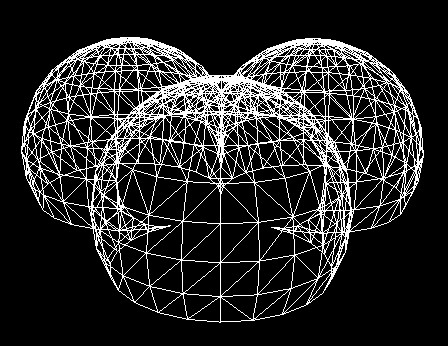
\includegraphics[width=3in]{balls.jpg}
			\label{figure.label}
		\end{center}
	\end{figure}
	\begin{figure}[htbp]
		\centering
		\begin{minipage}{0.24\linewidth}
			\centering
			\caption{cot,圆形边界}
			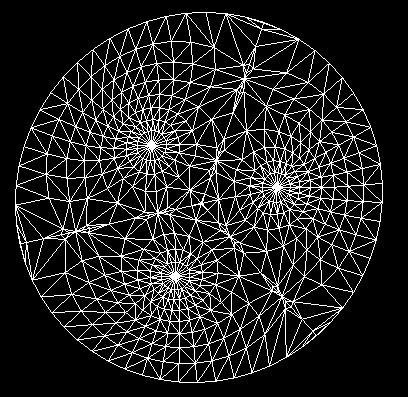
\includegraphics[width=1\linewidth]{balls_circle.JPG}
			\label{chutian1}%文中引用该图片代号
		\end{minipage}
		%\qquad
		\begin{minipage}{0.24\linewidth}
			\centering
			\caption{cot,正方形边界}
			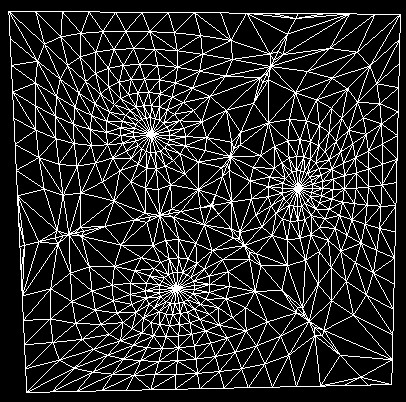
\includegraphics[width=1\linewidth]{balls_square.JPG}
			\label{chutian2}%文中引用该图片代号
		\end{minipage}
		%\qquad
		\begin{minipage}{0.24\linewidth}
			\centering
			\caption{ASAP参数化}
			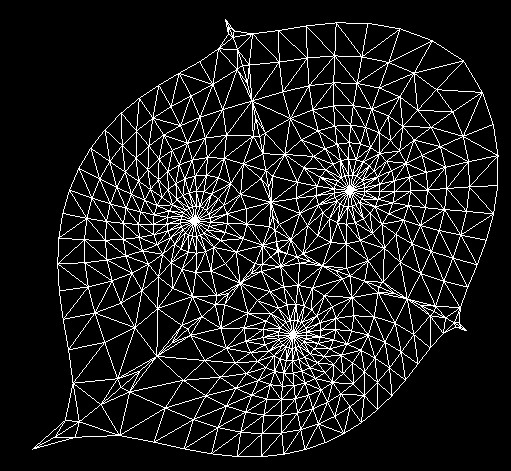
\includegraphics[width=1\linewidth]{balls_asap.JPG}
			\label{chutian2}%文中引用该图片代号
		\end{minipage}
		%\qquad
		\begin{minipage}{0.24\linewidth}
			\centering
			\caption{ARAP参数化}
			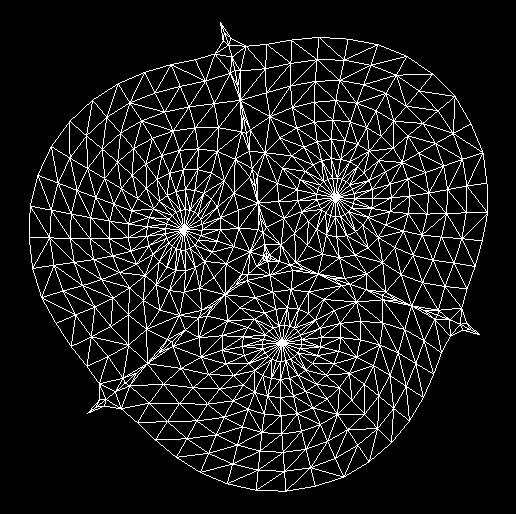
\includegraphics[width=1\linewidth]{balls_arap.JPG}
			\label{chutian2}%文中引用该图片代号
		\end{minipage}
	\end{figure}
	\begin{figure}[htbp]
		\centering
		\begin{minipage}{0.24\linewidth}
			\centering
			\caption{cot,圆形边界}
			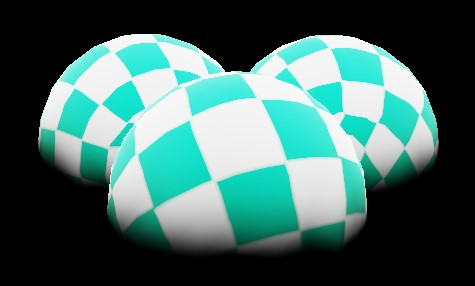
\includegraphics[width=1\linewidth]{balls_circle_tex.JPG}
			\label{chutian1}%文中引用该图片代号
		\end{minipage}
		%\qquad
		\begin{minipage}{0.24\linewidth}
			\centering
			\caption{cot,正方形边界}
			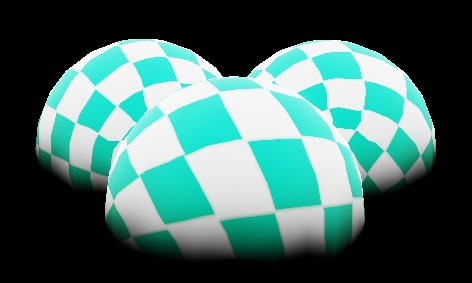
\includegraphics[width=1\linewidth]{balls_square_tex.JPG}
			\label{chutian2}%文中引用该图片代号
		\end{minipage}
		%\qquad
		\begin{minipage}{0.24\linewidth}
			\centering
			\caption{ASAP参数化}
			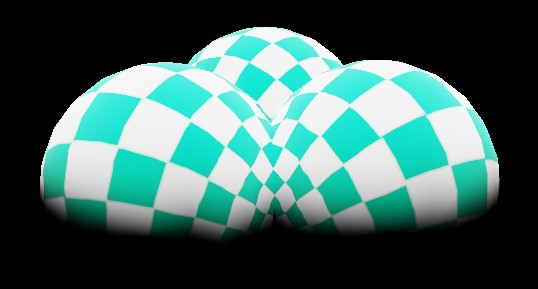
\includegraphics[width=1\linewidth]{balls_asap_tex.JPG}
			\label{chutian2}%文中引用该图片代号
		\end{minipage}
		%\qquad
		\begin{minipage}{0.24\linewidth}
			\centering
			\caption{ARAP参数化}
			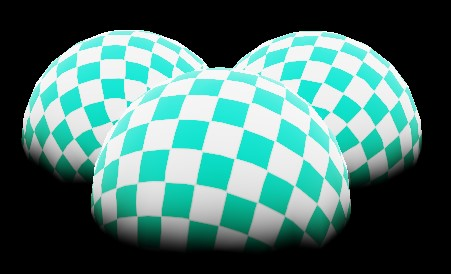
\includegraphics[width=1\linewidth]{balls_arap_tex.JPG}
			\label{chutian2}%文中引用该图片代号
		\end{minipage}
	\end{figure}
	\clearpage
	
	%cow
	\begin{figure}[htb]
		\caption{\label{table.label} cow原网格} \centering
		\begin{center}
			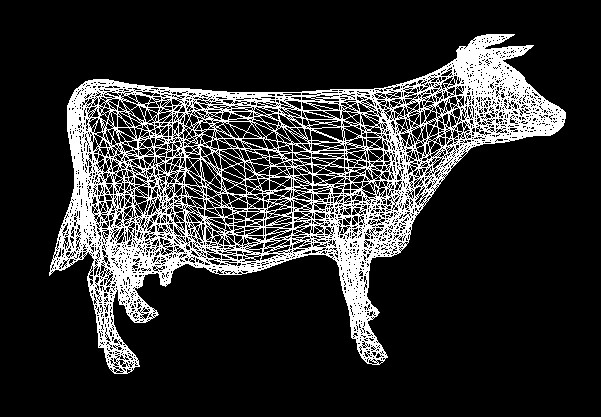
\includegraphics[width=2.2in]{cow.jpg}
			\label{figure.label}
		\end{center}
	\end{figure}
	\begin{figure}[htbp]
		\centering
		\begin{minipage}{0.49\linewidth}
			\centering
			\caption{ASAP参数化}
			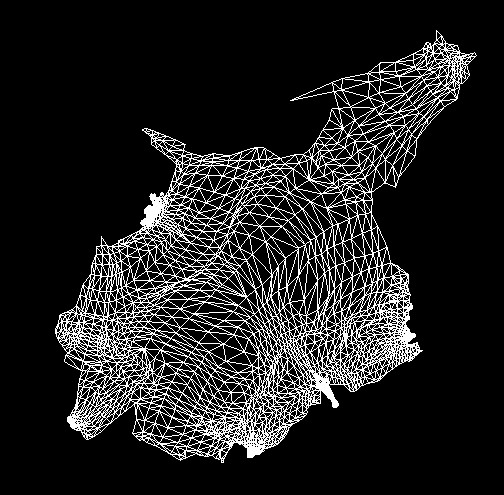
\includegraphics[width=0.8\linewidth]{cow_asap.JPG}
			\label{chutian2}%文中引用该图片代号
		\end{minipage}
		%\qquad
		\begin{minipage}{0.49\linewidth}
			\centering
			\caption{ARAP参数化}
			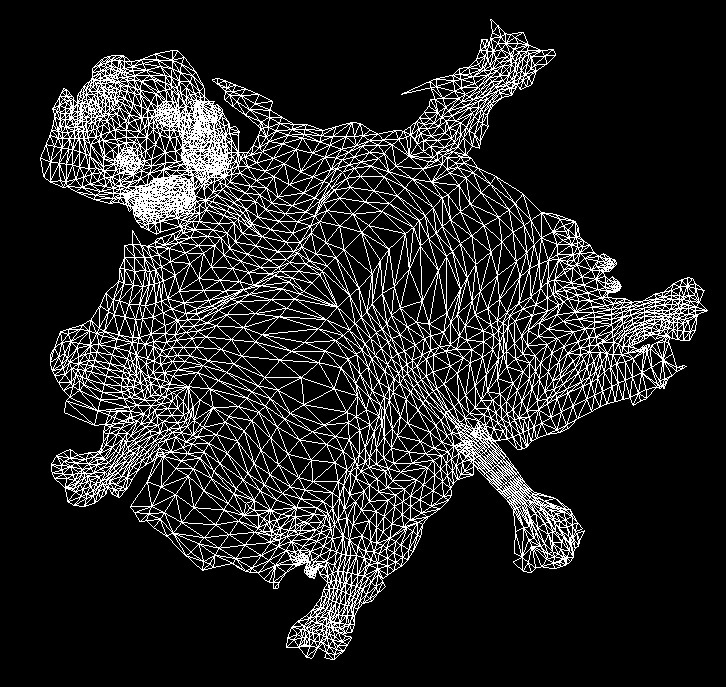
\includegraphics[width=0.8\linewidth]{cow_arap.JPG}
			\label{chutian2}%文中引用该图片代号
		\end{minipage}
	\end{figure}
	\begin{figure}[htbp]
		\centering
		\begin{minipage}{0.49\linewidth}
			\centering
			\caption{ASAP参数化}
			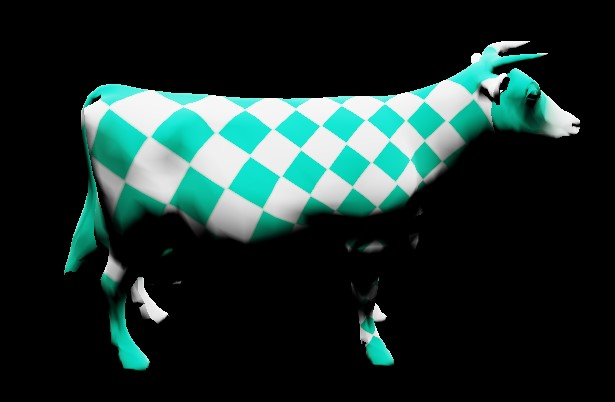
\includegraphics[width=0.7\linewidth]{cow_asap_tex.JPG}
			\label{chutian2}%文中引用该图片代号
		\end{minipage}
		%\qquad
		\begin{minipage}{0.49\linewidth}
			\centering
			\caption{ARAP参数化}
			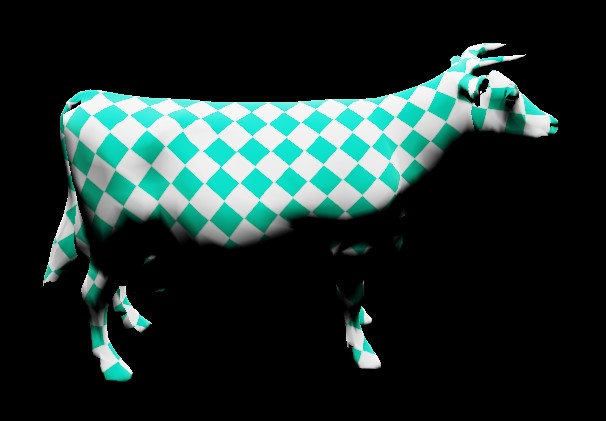
\includegraphics[width=0.7\linewidth]{cow_arap_tex.JPG}
			\label{chutian2}%文中引用该图片代号
		\end{minipage}
	\end{figure}
	\clearpage

	%beetle
	\begin{figure}[htb]
		\caption{\label{table.label} beetle原网格} \centering
		\begin{center}
			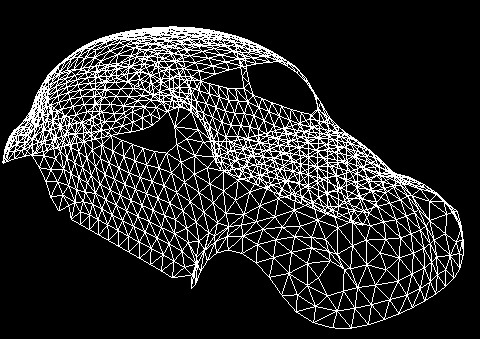
\includegraphics[width=2.2in]{beetle.jpg}
			\label{figure.label}
		\end{center}
	\end{figure}
	\begin{figure}[htbp]
		\centering
		\begin{minipage}{0.49\linewidth}
			\centering
			\caption{ASAP参数化}
			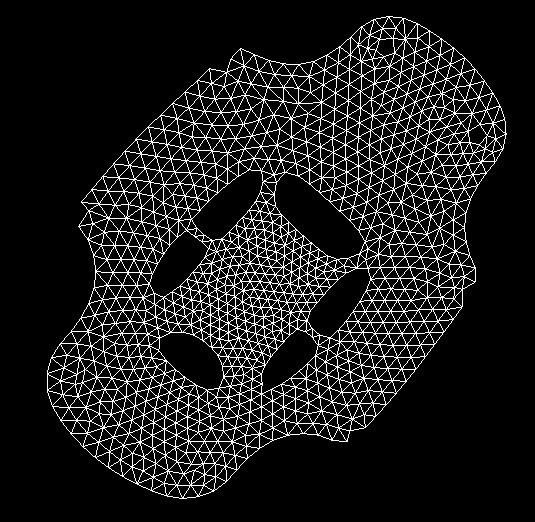
\includegraphics[width=0.8\linewidth]{beetle_asap.JPG}
			\label{chutian2}%文中引用该图片代号
		\end{minipage}
		%\qquad
		\begin{minipage}{0.49\linewidth}
			\centering
			\caption{ARAP参数化}
			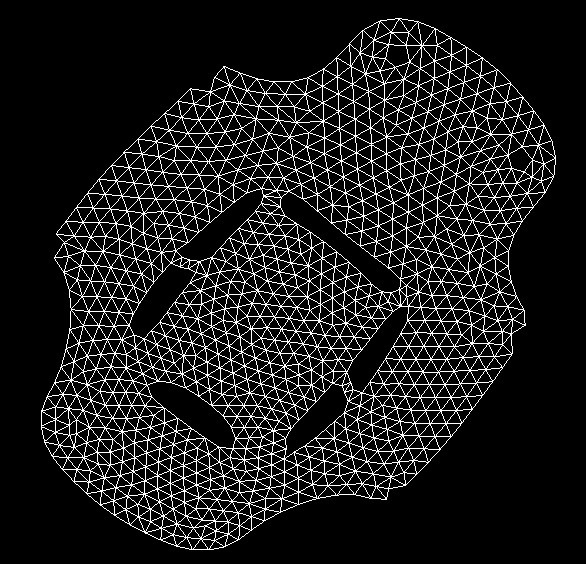
\includegraphics[width=0.8\linewidth]{beetle_arap.JPG}
			\label{chutian2}%文中引用该图片代号
		\end{minipage}
	\end{figure}
	\begin{figure}[htbp]
		\centering
		\begin{minipage}{0.49\linewidth}
			\centering
			\caption{ASAP参数化}
			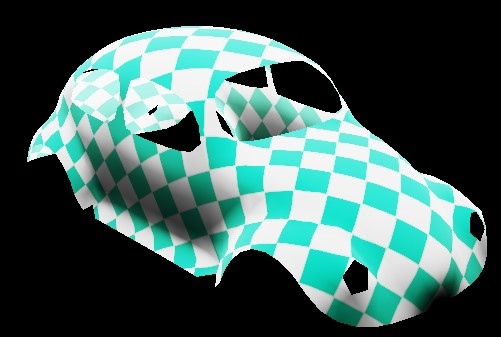
\includegraphics[width=0.7\linewidth]{beetle_asap_tex.JPG}
			\label{chutian2}%文中引用该图片代号
		\end{minipage}
		%\qquad
		\begin{minipage}{0.49\linewidth}
			\centering
			\caption{ARAP参数化}
			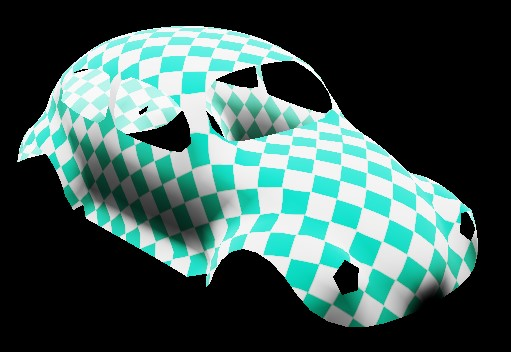
\includegraphics[width=0.7\linewidth]{beetle_arap_tex.JPG}
			\label{chutian2}%文中引用该图片代号
		\end{minipage}
	\end{figure}
	\clearpage

	%lsis
	\begin{figure}[htb]
		\caption{\label{table.label} lsis原网格} \centering
		\begin{center}
			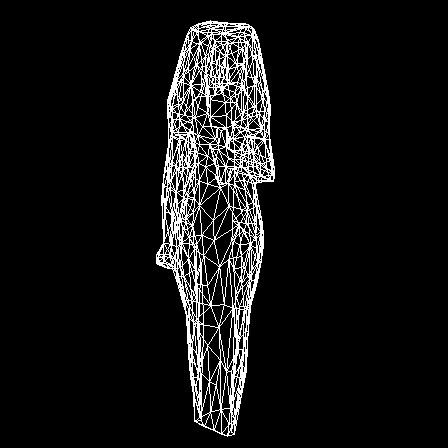
\includegraphics[width=2in]{lsis.jpg}
			\label{figure.label}
		\end{center}
	\end{figure}
	\begin{figure}[htbp]
		\centering
		\begin{minipage}{0.24\linewidth}
			\centering
			\caption{cot,圆形边界}
			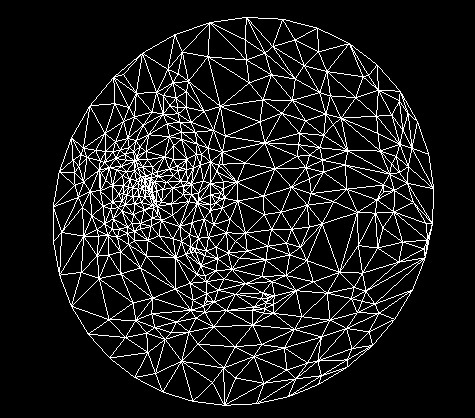
\includegraphics[width=1\linewidth]{lsis_circle.JPG}
			\label{chutian1}%文中引用该图片代号
		\end{minipage}
		%\qquad
		\begin{minipage}{0.24\linewidth}
			\centering
			\caption{cot,正方形边界}
			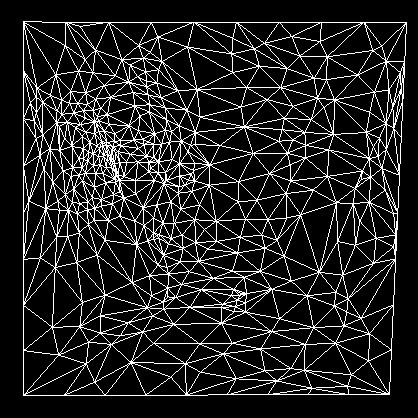
\includegraphics[width=1\linewidth]{lsis_square.JPG}
			\label{chutian2}%文中引用该图片代号
		\end{minipage}
		%\qquad
		\begin{minipage}{0.24\linewidth}
			\centering
			\caption{ASAP参数化}
			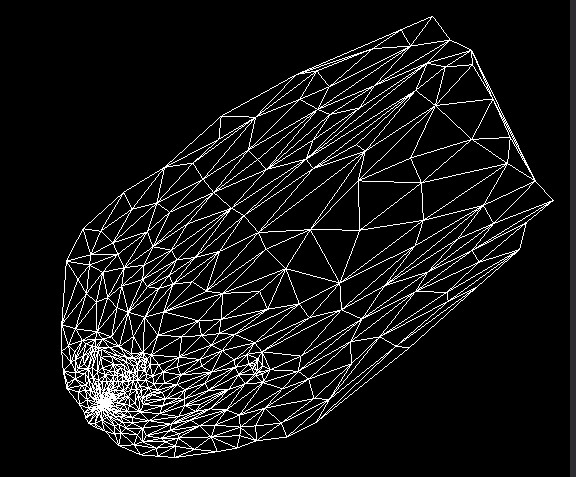
\includegraphics[width=1\linewidth]{lsis_asap.JPG}
			\label{chutian2}%文中引用该图片代号
		\end{minipage}
		%\qquad
		\begin{minipage}{0.24\linewidth}
			\centering
			\caption{ARAP参数化}
			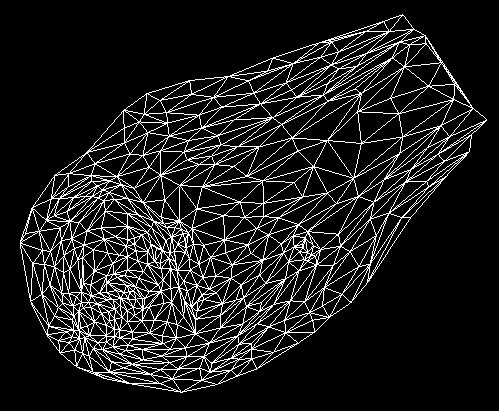
\includegraphics[width=1\linewidth]{lsis_arap.JPG}
			\label{chutian2}%文中引用该图片代号
		\end{minipage}
	\end{figure}
	\begin{figure}[htbp]
		\centering
		\begin{minipage}{0.24\linewidth}
			\centering
			\caption{cot,圆形边界}
			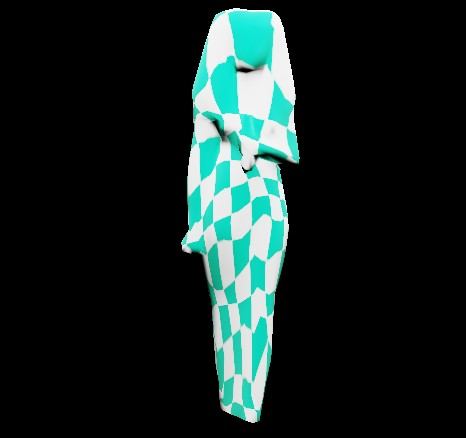
\includegraphics[width=1\linewidth]{lsis_circle_tex.JPG}
			\label{chutian1}%文中引用该图片代号
		\end{minipage}
		%\qquad
		\begin{minipage}{0.24\linewidth}
			\centering
			\caption{cot,正方形边界}
			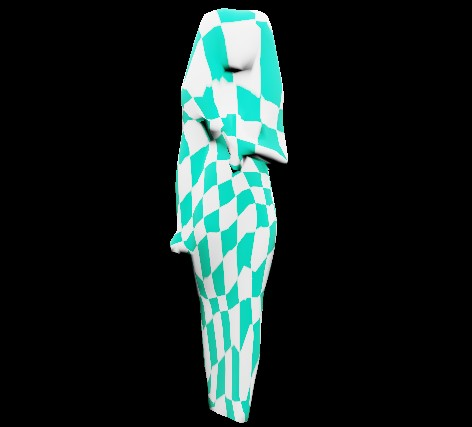
\includegraphics[width=1\linewidth]{lsis_square_tex.JPG}
			\label{chutian2}%文中引用该图片代号
		\end{minipage}
		%\qquad
		\begin{minipage}{0.24\linewidth}
			\centering
			\caption{ASAP参数化}
			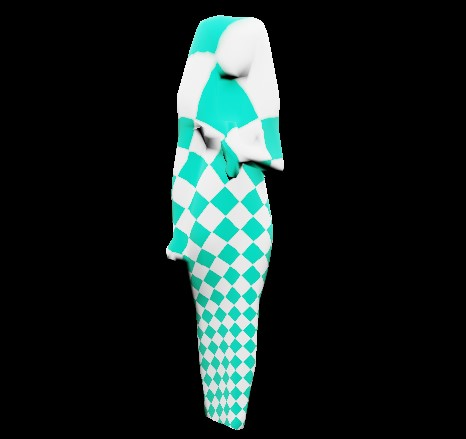
\includegraphics[width=1\linewidth]{lsis_asap_tex.JPG}
			\label{chutian2}%文中引用该图片代号
		\end{minipage}
		%\qquad
		\begin{minipage}{0.24\linewidth}
			\centering
			\caption{ARAP参数化}
			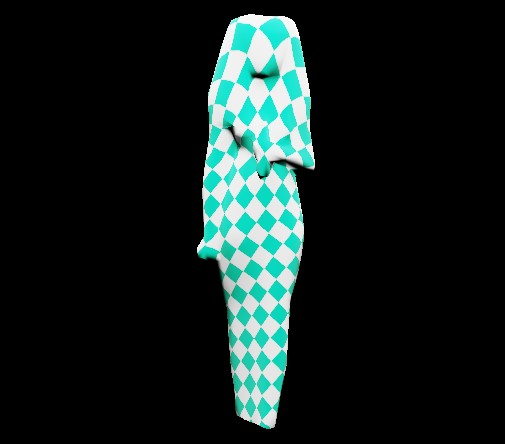
\includegraphics[width=1\linewidth]{lsis_arap_tex.JPG}
			\label{chutian2}%文中引用该图片代号
		\end{minipage}
	\end{figure}
	\clearpage

	%gargoyle
	\begin{figure}[htb]
		\caption{\label{table.label} gargoyle原网格} \centering
		\begin{center}
			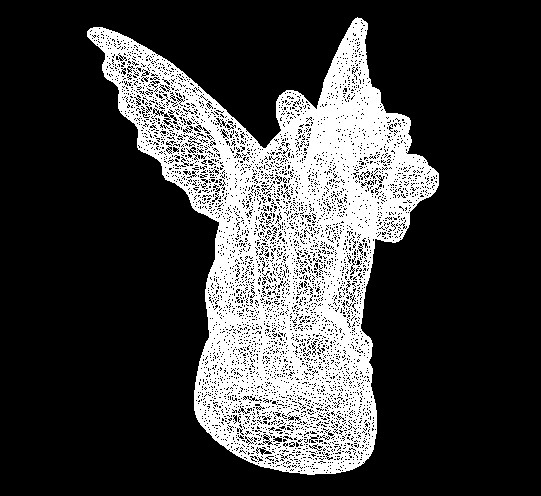
\includegraphics[width=2.2in]{gargoyle.jpg}
			\label{figure.label}
		\end{center}
	\end{figure}
	\begin{figure}[htbp]
		\centering
		\begin{minipage}{0.24\linewidth}
			\centering
			\caption{cot,圆形边界}
			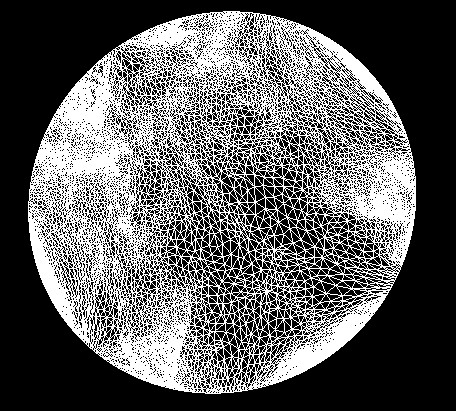
\includegraphics[width=1\linewidth]{gargoyle_circle.JPG}
			\label{chutian1}%文中引用该图片代号
		\end{minipage}
		%\qquad
		\begin{minipage}{0.24\linewidth}
			\centering
			\caption{cot,正方形边界}
			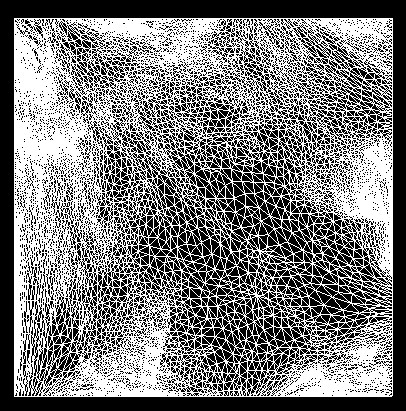
\includegraphics[width=1\linewidth]{gargoyle_square.JPG}
			\label{chutian2}%文中引用该图片代号
		\end{minipage}
		%\qquad
		\begin{minipage}{0.24\linewidth}
			\centering
			\caption{ASAP参数化}
			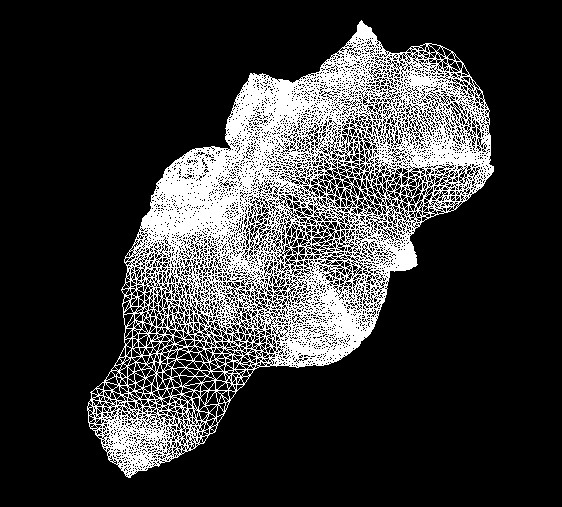
\includegraphics[width=1\linewidth]{gargoyle_asap.JPG}
			\label{chutian2}%文中引用该图片代号
		\end{minipage}
		%\qquad
		\begin{minipage}{0.24\linewidth}
			\centering
			\caption{ARAP参数化}
			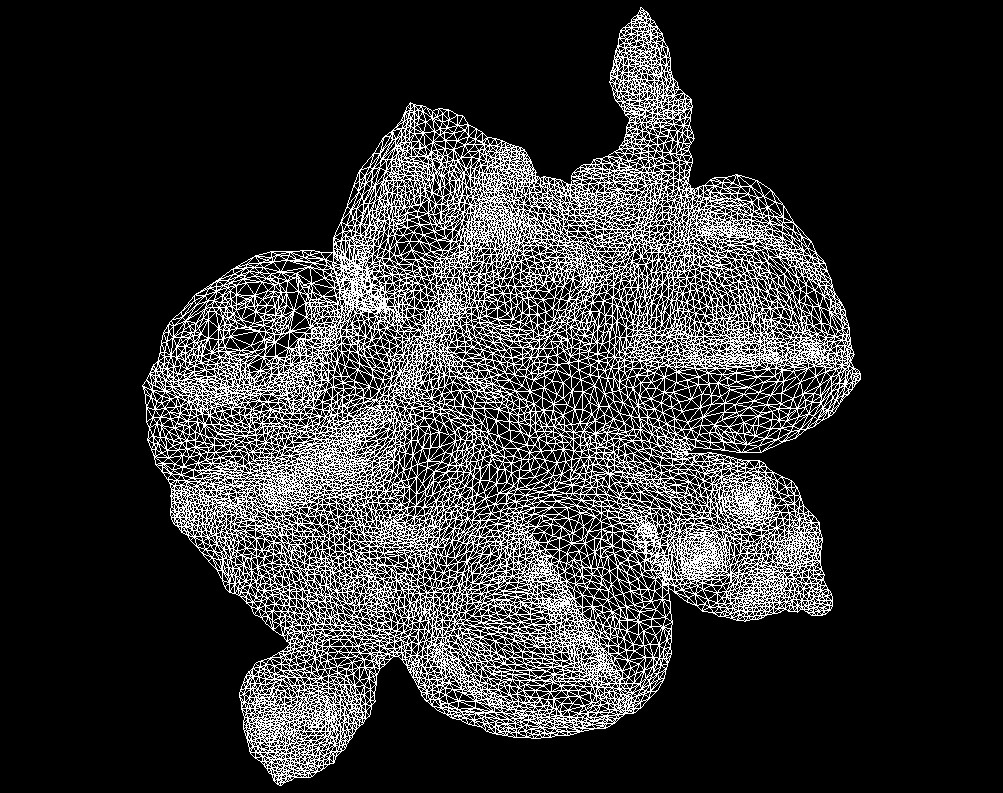
\includegraphics[width=1\linewidth]{gargoyle_arap.JPG}
			\label{chutian2}%文中引用该图片代号
		\end{minipage}
	\end{figure}
	\begin{figure}[htbp]
		\centering
		\begin{minipage}{0.24\linewidth}
			\centering
			\caption{cot,圆形边界}
			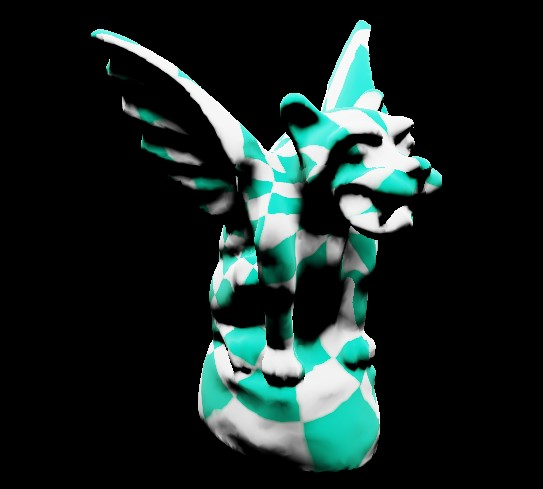
\includegraphics[width=1\linewidth]{gargoyle_circle_tex.JPG}
			\label{chutian1}%文中引用该图片代号
		\end{minipage}
		%\qquad
		\begin{minipage}{0.24\linewidth}
			\centering
			\caption{cot,正方形边界}
			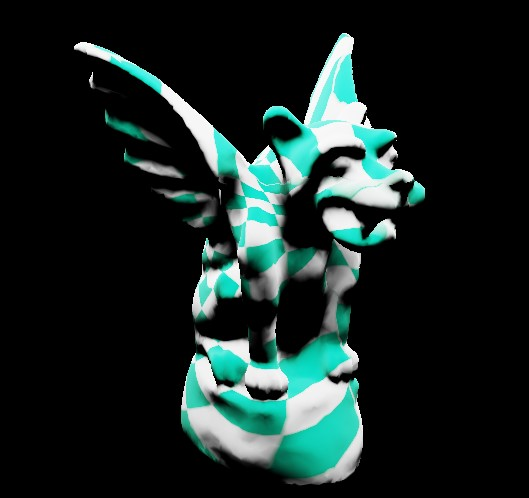
\includegraphics[width=1\linewidth]{gargoyle_square_tex.JPG}
			\label{chutian2}%文中引用该图片代号
		\end{minipage}
		%\qquad
		\begin{minipage}{0.24\linewidth}
			\centering
			\caption{ASAP参数化}
			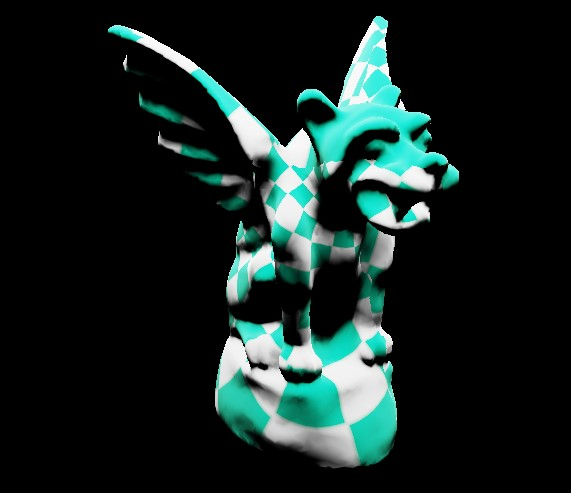
\includegraphics[width=1\linewidth]{gargoyle_asap_tex.JPG}
			\label{chutian2}%文中引用该图片代号
		\end{minipage}
		%\qquad
		\begin{minipage}{0.24\linewidth}
			\centering
			\caption{ARAP参数化}
			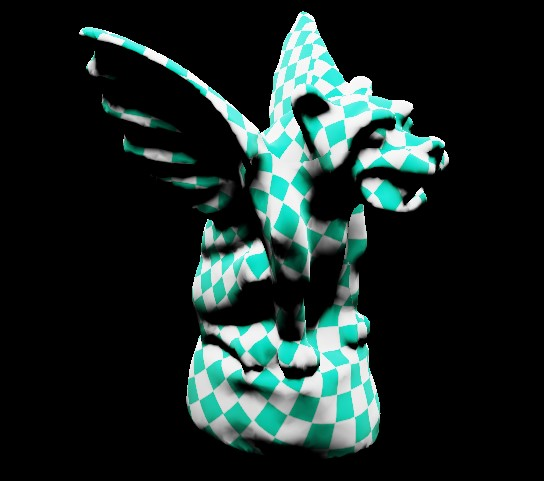
\includegraphics[width=1\linewidth]{gargoyle_arap_tex.JPG}
			\label{chutian2}%文中引用该图片代号
		\end{minipage}
	\end{figure}
	\clearpage
	
	在ARAP参数化中,我们采用设置了输入框和滑条,让用户给出ARAP参数化过程中的迭代次数(
	如下图)。
	\begin{figure}[htb]
		\caption{\label{table.label} 迭代次数的输入框和滑条} \centering
		\begin{center}
			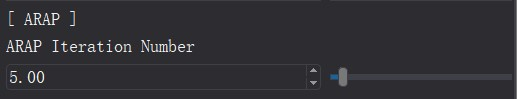
\includegraphics[width=4in]{iternum.jpg}
			\label{figure.label}
		\end{center}
	\end{figure}
	
	在实现算法的过程中,难点在于Laplace矩阵的构建需要比较细心。从上面的结果我们可以看到,
	效果最好的是ARAP参数化,纹理贴图中它的方块没有明显的扭曲,而且大小都相近。虽然ARAP
	参数化对初始参数化不是很敏感,但是采用ASAP参数化作为初始参数化会导致每次迭代后的变
	化不是很明显,即很容易就能达到精度较高的参数化。如果我们采用固定到正方形边界的参数
	化作为初始参数化,可能前几次迭代还会有较大变化,之后也能很快收敛到我们想要的网格。
\section{参考文献}
  $[1]$Ligang Liu,Lei Zhang,Yin Xu,Craig Gotsman,Steven J. Gortler,A 
  Local/Global Approach to Mesh Parameterization,Eurographics Symposium on 
  Geometry Processing 2008,Volume 27 (2008), Number 5
\end{document}
